\documentclass{article}
\usepackage{amsmath}
\usepackage{algpseudocode}
\usepackage{tikz}
\title{Bezier Shape Functions}
\author{Dan Zaide}
\date{Sep 12, 2015}
\begin{document}
\maketitle

\section{Bezier Curves}
The Bezier curve, $\mathbf{B}(t)$ of order $P$ is polynomial defined by the set of control points $\mathbf{C}_i$ for $i = 0,\ldots,P$ as 
\[
\mathbf{B}(t) = \displaystyle \sum_{i=0}^P {P \choose i}t^i(1-t)^{P-i}\mathbf{C}_i
\]
where ${P \choose i}= \frac{P!}{i!(P-i)!}$ is the binomial coefficient and $ t \in [0,1]$. The derivatives are
\[
\frac{\mathrm{d} \mathbf{B}(t)}{\mathrm{d} t} = \displaystyle \sum_{i=0}^P {P \choose i}(i-Pt)t^{i-1}(1-t)^{P-i-1}\mathbf{C}_i
\]
and
\[
\frac{\mathrm{d}^2 \mathbf{B}(t)}{\mathrm{d} t^2} = \displaystyle \sum_{i=0}^P {P \choose i}((P-1)Pt^2-2i(P-1)t+i(i-1))t^{i-2}(1-t)^{P-i-2}\mathbf{C}_i
\]
where
\[\left.\frac{\mathrm{d}^2 \mathbf{B}(t)}{\mathrm{d} t^2}\right|_t=0 = P(P-1)(\mathbf{C}_0-2\mathbf{C}_1+\mathbf{C}_2)\]
In the current implementation in \texttt{BezierShape} in \texttt{crvBezier.cc}, the edge shape functions are ordered with the vertices first, as $v_0,v_1,e_0,\ldots,e_{p-1}$, which is not geometric order.
\subsection{Interpolating Bezier Curves}
To fit a bezier curve to a known geometry, interpolating points, $\mathbf{P}_j = \mathbf{P}(t_j)$, are first needed at $t_0,\ldots, t_{P+1}$ before the control points can be solved for. This requires solving

\[
\mathbf{B}(t_j) = \displaystyle \sum_{i=0}^P {P \choose i}t_j^i(1-t_j)^{P-i}\mathbf{C}_i = \mathbf{P}_i
\]
at each interpolating point, resulting in a linear system of equations for $\mathbf{C}_i$. The following matlab code solves for these coefficients, which each row of $\mathbf{A}^{-1}$ corresponding to coefficients for the interpolating points. The first six orders are implemented in \texttt{convertEdgeLocations2D} and \texttt{convertEdgeLocations3D}.

Several choices of $t_j$ exist. Using equally spaced $t$'s works fairly well, but closer to optimal points are in \textit{Approximate optimal points for polynomial interpolation of real functions in an interval and in a triangle}, Chen and Babuska, 1995.
\section{Bezier Triangles}
The Bezier triangle is similar, with each edge its own Bezier curve. For an order $P$ triangle, there are $(P+1)(P+2)/2$ control points, with $(P-1)(P-2)/2$ points on the interior. Using barycentric coordinates $u,v,w = 1-u-v$ we can define the Bezier triangle as 
\[
\mathbf{B}(u,v) = \displaystyle\sum_{i,j,k\geq 0}^{i+j+k=P} \frac{P!}{i!j!k!}u^iv^jw^k \alpha^i\beta^j\gamma^k 
\]
where $\alpha^i\beta^j\gamma^k$ correspond to the control points. In our implementation, we use a finite element coordinate system where our parameters are $\xi_0,\xi_1$ and our triangle has vertex 0 at $1-\xi_0-\xi_1$, vertex 1 at $\xi_0$ and vertex 2 at $\xi_1$.

This is implemented in a single array with size $(P+1)(P+2)/2$. The summation is then rewritten as
\[
\mathbf{B}(u,v) = \displaystyle\sum_{i=0}^P \sum_{j=0}^{P-i}\frac{P!}{i!j!(P-i-j)!}u^iv^j(1-u-v)^{P-i-j}\mathbf{P}_\ell, \quad \ell = (P+1)j+i-j(j-1)/2
\]
In the actual implementation, vertices are the first three points, edges are the next $3(P-1)$ and faces are the rest. So our list of points is actually $v_0,v_1,v_2,e_{0,0},\ldots,e_{0,P-1},e_{1,0},\ldots,e_{1,P-1},e_{2,0},\ldots,e_{2,P-1},f_0,\ldots,f_{(P-1)(P-2)/2}$. 
\begin{figure}
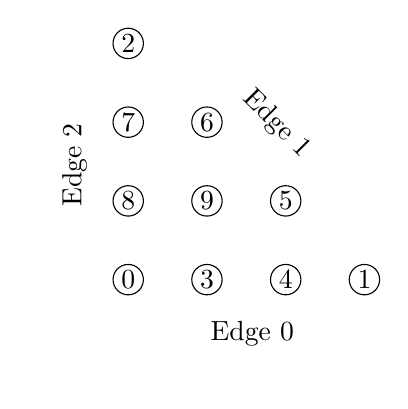
\begin{tikzpicture}[scale=1]
\tikzstyle{every node}=[circle, draw, fill=white,
                        inner sep=1pt, minimum width=5pt]
\path (0,0) node {$0$}
(1,0) node [label={[label distance=0.1cm]-60:Edge 0}] {$3$}
(2,0) node {$4$}
(3,0) node {$1$}
(2,1) node {$5$}
(1,2) node [label={[label distance=0.1cm,rotate=-45]10:Edge 1}] {$6$}
(0,3) node {$2$}
(0,2) node [label={[label distance=0.2cm,rotate=90]-200:Edge 2}] {$7$}
(0,1) node {$8$}
(1,1) node {$9$};

\end{tikzpicture} \hspace{1cm}
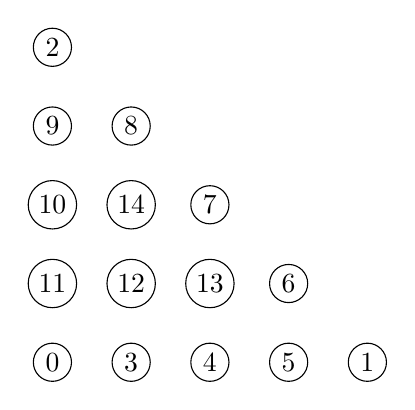
\begin{tikzpicture}[scale=1]
\tikzstyle{every node}=[circle, draw, fill=white,
                        inner sep=2pt, minimum width=5pt]
\path (0,0) node {$0$}
(1,0) node {$3$}
(2,0) node {$4$}
(3,0) node {$5$}
(4,0) node {$1$}
(3,1) node {$6$}
(2,2) node {$7$}
(1,3) node {$8$}
(0,4) node {$2$}
(0,3) node {$9$}
(0,2) node {$10$}
(0,1) node {$11$}
(1,1) node {$12$}
(2,1) node {$13$}
(1,2) node {$14$};

\end{tikzpicture} \\
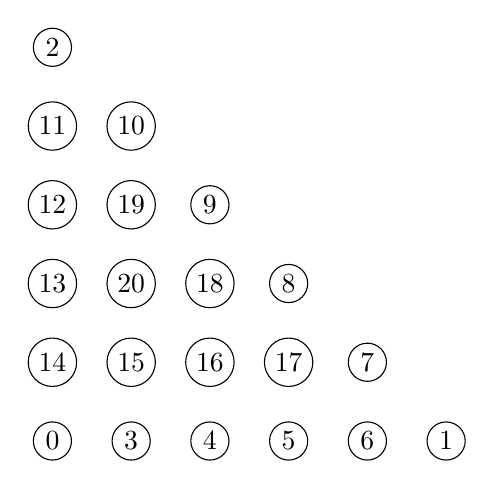
\begin{tikzpicture}[scale=1]
\tikzstyle{every node}=[circle, draw, fill=white,
                        inner sep=2pt, minimum width=5pt]
\path (0,0) node {$0$}
(1,0) node {$3$}
(2,0) node {$4$}
(3,0) node {$5$}
(4,0) node {$6$}
(5,0) node {$1$}
(4,1) node {$7$}
(3,2) node {$8$}
(2,3) node {$9$}
(1,4) node {$10$}
(0,5) node {$2$}
(0,4) node {$11$}
(0,3) node {$12$}
(0,2) node {$13$}
(0,1) node {$14$}
(1,1) node {$15$}
(2,1) node {$16$}
(3,1) node {$17$}
(2,2) node {$18$}
(1,3) node {$19$}
(1,2) node {$20$};

\end{tikzpicture}\hspace{1cm}
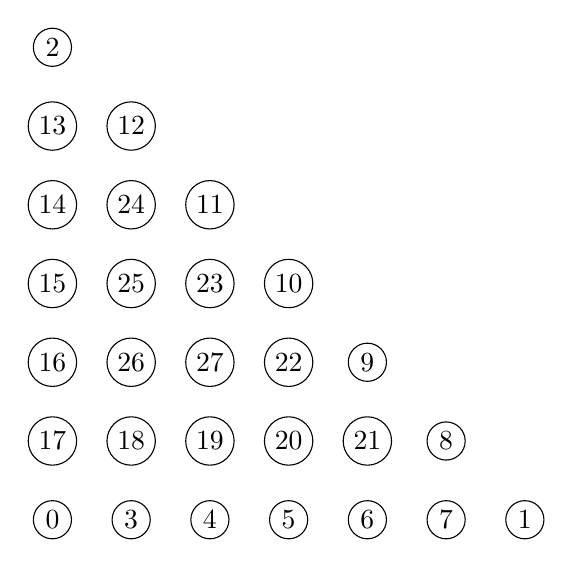
\begin{tikzpicture}[scale=1]
\tikzstyle{every node}=[circle, draw, fill=white,
                        inner sep=2pt, minimum width=5pt]
\path (0,0) node {$0$}
(1,0) node {$3$}
(2,0) node {$4$}
(3,0) node {$5$}
(4,0) node {$6$}
(5,0) node {$7$}
(6,0) node {$1$}
(5,1) node {$8$}
(4,2) node {$9$}
(3,3) node {$10$}
(2,4) node {$11$}
(1,5) node {$12$}
(0,6) node {$2$}
(0,5) node {$13$}
(0,4) node {$14$}
(0,3) node {$15$}
(0,2) node {$16$}
(0,1) node {$17$}
(1,1) node {$18$}
(2,1) node {$19$}
(3,1) node {$20$}
(4,1) node {$21$}
(3,2) node {$22$}
(2,3) node {$23$}
(1,4) node {$24$}
(1,3) node {$25$}
(1,2) node {$26$}
(2,2) node {$27$};

\end{tikzpicture}
\caption{Node ordering for 3-6 order bezier}
\end{figure}


This is much harder to write in index form, so in the implementation. this ordering is stored as a map, and called upon when getting values or local gradients. The gradients are easily computed as 
\begin{eqnarray*}
\frac{\partial \mathbf{B}(u,v)}{\partial u} &=& \displaystyle\sum_{i=0}^P \sum_{j=0}^{P-i}\frac{P!}{i!j!(P-i-j)!}((1-v)i-(P-j)u)u^{i-1}v^j(1-u-v)^{P-i-j-1}\mathbf{P}_\ell \\
\frac{\partial \mathbf{B}(u,v)}{\partial v} &=& \displaystyle\sum_{i=0}^P \sum_{j=0}^{P-i}\frac{P!}{i!j!(P-i-j)!}((1-u)j-(P-i)v)u^{i}v^{j-1}(1-u-v)^{P-i-j-1}\mathbf{P}_\ell
\end{eqnarray*}
which, in their current implementation are not valid when any $u,v,w = 0$, since this leads to $0^{-1}$.
\subsection{Triangular Blending}
For faces not on a boundary, triangular blending of shape functions is needed. This occurs for all 2D triangles and 3D interior triangles with an edge or more on the boundary. For a given entity on the mesh, we have a coordinate field such that 
\[ \mathbf{x}(\xi) = \sum_{i=0}^N w_i(\xi) \cdot \mathbf{x}_i \]
for an entity with $N$ total nodes, where $\xi = (u,v,w) = (\xi_0,\xi_1,\xi_2)$ and $\xi_2 = 1-\xi_0-\xi_1$. To implement the blending in our framework, we have 
\[\mathbf{x}_{face}(\xi) = \sum_{i=0}^{3}||\xi_{e_i}||\sum_{j=0}^{N_{edge}}w_{e_i,j}(\xi_{e_i})\cdot\mathbf{x}_{e_i,j}- \sum_{i=0}^{3}\xi_i\mathbf{x}_{v_i}\]
Where the edge parameters are
\begin{eqnarray*} 
\xi_{e_0} & = & \frac{\xi_1}{\xi_0+\xi_1},\quad ||\xi_{e_0}|| = \xi_0+\xi_1 \\
\xi_{e_1} & = & \frac{\xi_2}{\xi_1+\xi_2},\quad ||\xi_{e_1}|| = \xi_1+\xi_2 \\
\xi_{e_2} & = & \frac{\xi_0}{\xi_2+\xi_0},\quad ||\xi_{e_2}|| = \xi_2+\xi_0 
\end{eqnarray*}
Based on the canonical ordering of edges and faces. When any of $||\xi_{e_i}|| = 0$, we are either on a vertex opposite that edge, or on a different edge, and do not consider the contribution of those edges (avoiding dividing by zero).

The goal is then to find face weights such that \[\mathbf{x}_{face}(\xi) = \sum_{i=0}^{N_{face}} w_i(\xi) \cdot \mathbf{x}_i = \sum_{i=0}^{3}||\xi_{e_i}||\sum_{j=0}^{N_{edge}}w_{e_i,j}(\xi_{e_i})\cdot\mathbf{x}_{e_i,j}- \sum_{i=0}^{3}\xi_i\mathbf{x}_{v_i} \] 
This is a bookkeeping exercise, since every $x_{e_i,j}$ corresponds to a point on the face, in $x_i$. Consider the third-order triangle, and its edges. The middle point is present, but excluded in the blending.
\begin{figure}
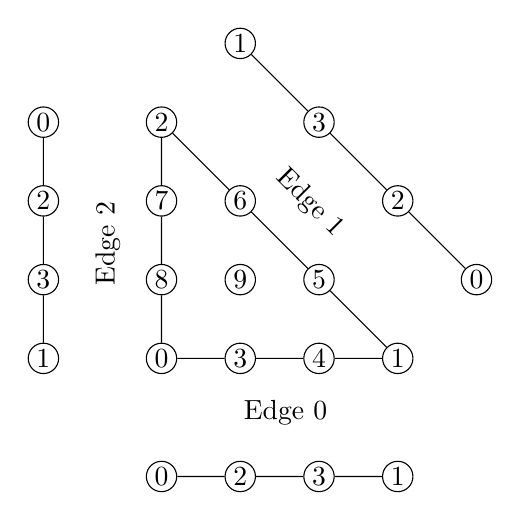
\begin{tikzpicture}[scale=1]
\tikzstyle{every node}=[circle, draw, fill=white,
                        inner sep=1pt, minimum width=4pt]
\path (0,0) node (p0) {$0$}
(1,0) node [label={[label distance=0.1cm]-60:Edge 0}] (p1) {$3$}
(2,0) node (p2) {$4$}
(3,0) node (p3) {$1$}
(2,1) node (p4) {$5$}
(1,2) node [label={[label distance=0.1cm,rotate=-45]10:Edge 1}] (p5) {$6$}
(0,3) node (p6) {$2$}
(0,2) node [label={[label distance=0.2cm,rotate=90]-200:Edge 2}] (p7) {$7$}
(0,1) node (p8) {$8$}
(1,1) node (p9) {$9$}
(0,-1.5) node (p10) {$0$}
(1,-1.5) node (p11) {$2$}
(2,-1.5) node (p12) {$3$}
(3,-1.5) node (p13) {$1$}
(-1.5,0) node (p14) {$1$}
(-1.5,1) node (p15) {$3$}
(-1.5,2) node (p16) {$2$}
(-1.5,3) node (p17) {$0$}
(1,4) node (p18) {$1$}
(2,3) node (p19) {$3$}
(3,2) node (p20) {$2$}
(4,1) node (p21) {$0$};
\draw (p0) -- (p1)
(p1) -- (p2)
(p2) -- (p3)
(p3) -- (p4)
(p4) -- (p5)
(p5) -- (p6)
(p6) -- (p7)
(p7) -- (p8)
(p8) -- (p0)
(p10) -- (p11)
(p11) -- (p12)
(p12) -- (p13)
(p14) -- (p15)
(p15) -- (p16)
(p16) -- (p17)
(p18) -- (p19)
(p19) -- (p20)
(p20) -- (p21);
\end{tikzpicture}
\end{figure}
The face has 9 nodes associated with it, ordered as shown. The weights are then 
\begin{eqnarray*}
w_0 & = & ||\xi_{e_0}||w_{e_0,0}(\xi_{e_0}) + ||\xi_{e_2}||w_{e_2,1}(\xi_{e_2}) - \xi_0 \\
w_1 & = & ||\xi_{e_0}||w_{e_0,1}(\xi_{e_0}) + ||\xi_{e_1}||w_{e_1,0}(\xi_{e_1}) - \xi_1 \\
w_2 & = & ||\xi_{e_2}||w_{e_2,0}(\xi_{e_2}) + ||\xi_{e_1}||w_{e_1,1}(\xi_{e_1}) - \xi_2 \\
w_3 & = & ||\xi_{e_0}||w_{e_0,2}(\xi_{e_0}) \\
w_4 & = & ||\xi_{e_0}||w_{e_0,3}(\xi_{e_0}) \\
w_5 & = & ||\xi_{e_1}||w_{e_1,2}(\xi_{e_1}) \\
w_6 & = & ||\xi_{e_1}||w_{e_1,3}(\xi_{e_1}) \\
w_7 & = & ||\xi_{e_2}||w_{e_2,2}(\xi_{e_2}) \\
w_8 & = & ||\xi_{e_2}||w_{e_2,3}(\xi_{e_2}) \\
w_9 & = & 0
\end{eqnarray*}
The local gradients are then
\begin{eqnarray*}\frac{\partial \mathbf{x}(\xi)}{\partial \xi_k}& = & \sum_{i=0}^N \frac{\partial w_i(\xi)}{\partial \xi_k} \cdot \mathbf{x}_i \\
\frac{\partial \mathbf{x}(\xi)}{\partial \xi_k}& = & \frac{\partial}{\partial \xi_k}\left[\sum_{i=0}^{3}||\xi_{e_i}||\sum_{j=0}^{N_{edge}}w_{e_i,j}(\xi_{e_i})\cdot\mathbf{x}_{e_i,j}- \sum_{i=0}^{3}\xi_i\mathbf{x}_{v_i}\right] \\ & & 
\sum_{i=0}^{3}\frac{\partial}{\partial \xi_k}\left[||\xi_{e_i}||\sum_{j=0}^{N_{edge}}w_{e_i,j}(\xi_{e_i})\right]\cdot\mathbf{x}_{e_i,j}- \sum_{i=0}^{3} \frac{\partial \xi_i}{\partial \xi_k}\mathbf{x}_{v_i}\end{eqnarray*}
For the vertex terms, we have
\[ \frac{\partial \xi_i}{\partial \xi_k} = \left[ \begin{array}{ccc} 1 & 0 & 0 \\ 0 & 1 & 0 \\ -1 & -1 & 0 \end{array}\right]\]
and for the edge terms, the chain rule leads to
\begin{eqnarray*}\frac{\partial}{\partial \xi_k}\left[||\xi_{e_i}||\sum_{j=0}^{N_{edge}}w_{e_i,j}(\xi_{e_i})\right] & = & \frac{\partial ||\xi_{e_i}||}{\partial \xi_k}\sum_{j=0}^{N_{edge}}w_{e_i,j}(\xi_{e_i}) + ||\xi_{e_i}||\sum_{j=0}^{N_{edge}}\frac{\partial w_{e_i,j}(\xi_{e_i})}{\partial \xi_k}

\end{eqnarray*}
where the first term is straight forward, and the second term, 
\begin{eqnarray*}
||\xi_{e_i}||\frac{\partial w_{e_i,j}(\xi_{e_i})}{\partial \xi_k} & = & 
||\xi_{e_i}||\frac{\partial w_{e_i,j}(\xi_{e_i})}{\partial \xi_{e_i}}\frac{\partial \xi_{e_i}}{\partial \xi_k} \\ & = & 
||\xi_{e_i}||\frac{\partial w_{e_i,j}(\xi_{e_i})}{\xi_{e_i}}\left[\frac{\partial \xi_{e_i}'}{\partial \xi_k}||\xi_{e_i}||-\xi_{e_i}'\frac{\partial ||\xi_{e_i}||}{\partial \xi_k} \right]

\end{eqnarray*}
This can all be put together to form the derivative of the triangle blending. Both values and gradients are implemented in a generic form, using the triangle-edge ordering in \texttt{apfMesh.cc} to determine weights and coefficients on the weight terms. 

\subsection{Align Shared Nodes}
When obtaining the nodes for a particular triangle, specific ordering must be considered. This is due to edges not necessarily being oriented with the face. In \texttt{alignSharedNodes}, this problem is addressed by using \texttt{getAlignment} and specifying the order. If an edge is flipped with respect to the triangle, the ordering of the edge nodes is reversed and the correct ordering of nodes for the triangle is obtained.

\subsection{Split Point Locations on Triangles}
Given barycentric coordinates $u,v,w=1-u-v$ such that on a triangle in parameter space, $\mathbf{p} = u\mathbf{p}_0 + v\mathbf{p}_1 + w\mathbf{p}_2$ we are interested in splitting it at a given $(u,v,w)$. Due to denegeracy and periodicity, lets define this as a pair of linear splits, such that $ \mathbf{q} = a\mathbf{p}_0 + (1-a)\mathbf{p}_1 $ and $\mathbf{p} = b\mathbf{p}_2 + (1-b)\mathbf{q}$. Solving for $(a,b)$ gives $ a = v/(u+v), b = 1-u-v$. This is implemented in \texttt{crvSnap.cc}.

\subsection{Align Shared Nodes}
Ordering of edge nodes is the same as for a triangle, reversing them if they are flipped relative to the tetrahedron. For the face nodes in the tetrahedron, these can be flipped and rotated. The correct re-ordering is implemented in a more general form, but uses the fact the interior nodes form loops around the vertices, and rotation is just a shift by the number of nodes per edge. Flipped faces are less obvious, but the correct ordering is obtained by simply examining the flipped triangle's nodes, and matching the ordering (in the example below, node 6 is where node 0 is in the canonical triangle, so the ordering starts with 6). Examples are shown below.
\begin{figure}[!ht]
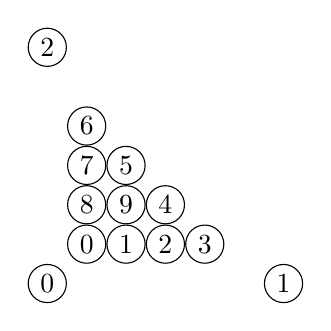
\begin{tikzpicture}[scale=0.5]
\tikzstyle{every node}=[circle, draw, fill=white,
                        inner sep=2pt, minimum width=5pt]
\path (0,0) node {$0$}

(6,0) node {$1$}
(0,6) node {$2$}
(1,1) node {$0$}
(2,1) node {$1$}
(3,1) node {$2$}
(4,1) node {$3$}
(3,2) node {$4$}
(2,3) node {$5$}
(1,4) node {$6$}
(1,3) node {$7$}
(1,2) node {$8$}
(2,2) node {$9$};

\end{tikzpicture}\hspace{0.5cm}
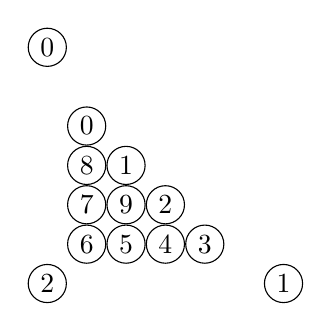
\begin{tikzpicture}[scale=0.5]
\tikzstyle{every node}=[circle, draw, fill=white,
                        inner sep=2pt, minimum width=5pt]
\path (0,0) node {$2$}

(6,0) node {$1$}
(0,6) node {$0$}
(1,1) node {$6$}
(2,1) node {$5$}
(3,1) node {$4$}
(4,1) node {$3$}
(3,2) node {$2$}
(2,3) node {$1$}
(1,4) node {$0$}
(1,3) node {$8$}
(1,2) node {$7$}
(2,2) node {$9$};
\end{tikzpicture}\hspace{0.5cm}
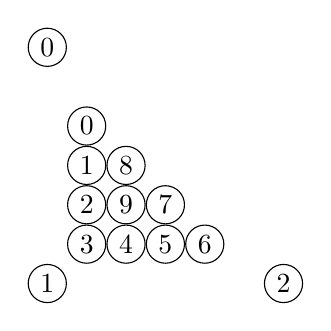
\begin{tikzpicture}[scale=0.5]
\tikzstyle{every node}=[circle, draw, fill=white,
                        inner sep=2pt, minimum width=5pt]
\path (0,0) node {$1$}
(6,0) node {$2$}
(0,6) node {$0$}
(1,1) node {$3$}
(2,1) node {$4$}
(3,1) node {$5$}
(4,1) node {$6$}
(3,2) node {$7$}
(2,3) node {$8$}
(1,4) node {$0$}
(1,3) node {$1$}
(1,2) node {$2$}
(2,2) node {$9$};
\end{tikzpicture}
\caption{Shared nodes for 6th order Bezier triangle. Original Ordering (left) (0,...,9). Flipped ordering (middle) (6,5,4,3,2,1,0,8,7,9). Rotated ordering by 2 (right) (3,4,5,6,7,8,0,1,2,9).}
\end{figure}

\section{G1 Gregory Patches}
G1 continuous patches are implemented following Walton and Meek, \textit{A triangular G1 patch from boundary curves}. The mesh is initially set to 4th order, with 6 face nodes for the G1 patch. First, all edges on a geometric surface have control points set (the first two nodes of the three) using surface normals and the vertex locations. Edges on geometric edges have their control points set using the tangents at their endpoints. These edge control points use the algorithm of Walton and Meek to set the six face nodes. Once the internal points are determined, the edges are formally elevated, by resetting all of the points to the elevated control points.

The weights on these nodes are similar to the triangular Bezier, with the evaluation done as if it is a Bezier triangle with internal Bezier points, $\mathbf{B}$, and Gregory points, $\mathbf{G}$.
\begin{equation}
\mathbf{B}_{12} = \frac{1}{\xi_1+\xi_2}(\xi_2\mathbf{G}_{12}+\xi_1\mathbf{G}_{17})
\end{equation}
\begin{equation}
\mathbf{B}_{13} = \frac{1}{\xi_0+\xi_2}(\xi_0\mathbf{G}_{13}+\xi_2\mathbf{G}_{15})
\end{equation}
\begin{equation}
\mathbf{B}_{14} = \frac{1}{\xi_0+\xi_1}(\xi_1\mathbf{G}_{14}+\xi_0\mathbf{G}_{16})
\end{equation}
The remainder of the mathematics is the same as the Bezier triangle, with tetrahedral blending, and other aspects maintaining the same form. We should note that choosing $\mathbf{G}_{12} = \mathbf{G}_{17}, \mathbf{G}_{13} = \mathbf{G}_{15}, \mathbf{G}_{14} = \mathbf{G}_{16}$ results in the original Bezier triangle, albeit with three additional nodes stored per triangle.
\begin{figure}
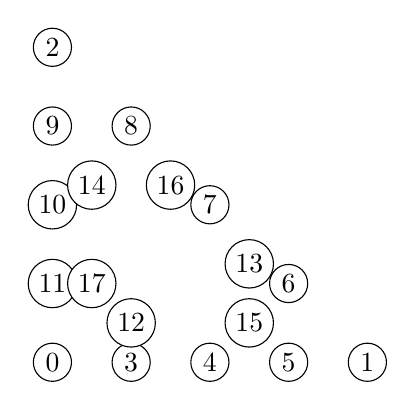
\begin{tikzpicture}[scale=1]
\tikzstyle{every node}=[circle, draw, fill=white,
                        inner sep=2pt, minimum width=5pt]
\path (0,0) node {$0$}
(1,0) node {$3$}
(2,0) node {$4$}
(3,0) node {$5$}
(4,0) node {$1$}
(3,1) node {$6$}
(2,2) node {$7$}
(1,3) node {$8$}
(0,4) node {$2$}
(0,3) node {$9$}
(0,2) node {$10$}
(0,1) node {$11$}
(1.0,0.5) node {$12$}
(2.5,1.25) node {$13$}
(0.5,2.25) node {$14$}
(2.5,0.5) node {$15$}
(1.5,2.25) node {$16$}
(0.5,1.0) node {$17$};

\end{tikzpicture} \hspace{2cm}
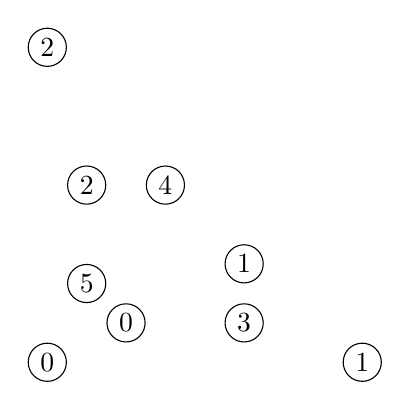
\begin{tikzpicture}[scale=1]
\tikzstyle{every node}=[circle, draw, fill=white,
                        inner sep=2pt, minimum width=5pt]
\path (0,0) node {$0$}

(4,0) node {$1$}

(0,4) node {$2$}

(1.0,0.5) node {$0$}
(2.5,1.25) node {$1$}
(0.5,2.25) node {$2$}
(2.5,0.5) node {$3$}
(1.5,2.25) node {$4$}
(0.5,1.0) node {$5$};

\end{tikzpicture}
\caption{Global and local node ordering for the 4th order G1 triangle. The ordering is chosen as these points are set based on edges, so node 0 and node 3 correspond to edge 0 and so forth.}
\end{figure}

\section{Tetrahedral Blending}
See papers by Dey and Shephard for more details. This is an extension of triangular blending. We use the finite element notation of $\xi = (1-\xi_0-\xi_1-\xi_2,\xi_0,\xi_1,\xi_2)$ rather than strict barycentrics. For a given entity on the mesh, we have a coordinate field such that 
\[ \mathbf{x}(\xi) = \sum_i w_i(\xi) \cdot \mathbf{x}_i \]
For tetrahedral blending, we then have that
\[\mathbf{x}(\xi) = \sum_{i=0}^{4}||\xi_{f_i}||w_{f_i}(\xi_{f_i})\mathbf{x}(\xi_{f_i}) - \sum_{i=0}^{6}||\xi_{e_i}||w_{e_i}(\xi_{e_i})\mathbf{x}(\xi_{e_i}) + \sum_{i=0}^{4}\xi_i\mathbf{x}_{v_i}\]
The weights for the tetrahedron are then obtained by summing corresponding weights from the faces, edges, and vertices. Similar to the triangle, we have the ordering of nodes on the tetrahedron as $v_0,v_1,v_2,v_3,[e_0],\ldots,[e_5],[f_0],\ldots,[f_3]$. Each edge and face is then called for its weights, and they are added into into the weights of the tetrahedron. For edges, this is straight-forward and identical to triangle blending. For triangles, the weights obtained also contain weights for the edges which must be added in, as well as the vertex weights. This is identified in the 
\texttt{tet\_tri\_edges}, containing the edges of the tetrahedron for each face. For example, face 2 is formed from vertices 1,2,3. On the tetrahedron, that corresponds to edges 1,5,4, with 4 in reverse order. Thus when adding to the weights of the edge nodes, if the edge is reversed, the weights are added in reverse order to the tetrahedron weight array, adding them to the correct index in the weight array.

Derivatives are computed identically to triangular blending, with multiple uses of the chain rule. Once again, when any of $||\xi_{e_i}||,||\xi_{f_i}|| = 0$, we do not consider the contribution of that entity.

\section{Bezier Tetrahedra}


\section{Bezier Elevation}
Given a Bezier curve of order $P$ with $P+1$ points, a curve of order $P+r$ can be computed, with point locations
\[
	\mathbf{C}_{i,P+r} = \displaystyle\sum_{j = \max(0,i-r)}^{\min(i,n)} \mathbf{C}_j {P \choose j} \frac{{r \choose i-j}}{{P+r \choose i}}
\]

\end{document}
